%%%%%%%%%%%%%%%%%%%%%%%%%%%%%%%%%%%%%%%%%

\chapter{The LANL nEDM experiment}\label{chap:LANL_nEDM}

%%%%%%%%%%%%%%%%%%%%%%%%%%%%%%%%%%%%%%%%%

At the Los Alamos National Laboratory (LANL), a solid deuterium (SD$_2$) based superthermal UCN source coupled to a spallation target has been providing UCN to experiments for the last 20 years (Fig.~\ref{fig:AreaB_schematic}). The UCN source (Sec.~\ref{sec:lanl_ucn_source}) was upgraded to host a new nEDM experiment that will use Ramsey's method of separated oscillatory fields to search for the nEDM with an uncertainty goal of $\delta \gls*{d_n} = 2.7\times 10^{-27}$~$e\cdot\text{cm}$ (Sec.~\ref{sec:lanl_nedm_uncertainty}).

The final LANL nEDM experiment will include features such as:
%
\begin{itemize}
    \item Two precession chambers (Sec.~\ref{sec:precession_chambers})
    \item Simultaneous spin analyzers (Sec.~\ref{sec:spin_flipper_analyzer})
    \item An external array of optically pumped magnetometers (Sec.~\ref{sec:magnetic_field_req})
    \item A $\ce{^{199}Hg}$ comagnetometer (Sec.~\ref{sec:199hg_comag}) and external $\ce{^{199}Hg}$ magnetometers
\end{itemize}

In this chapter we provide an overview of LANL nEDM components, and review some of the main systematic effects limiting the sensitivity of nEDM measurements.

%%%%%%%%%%%%%%%%%%%%%%%%%%%%%%%%%%%%%%%%%

\section{Principles of an nEDM measurement}\label{sec:principles_nEDM}

%%%%%%%%%%%%%%%%%%%%%%%%%%%%%%%%%%%%%%%%%

A measurement cycle in the envisioned LANL nEDM experiment consists of the following steps: 
%
\begin{enumerate}
    \item Polarized \ucn are loaded into precession cell(s), in a region where a static magnetic $\vv{B}_0$ and electric field $\vv{E}$ are applied. $\vv{B}_0$ and $\vv{E}$ are in either a parallel ($\uparrow\uparrow$) or antiparallel ($\uparrow\downarrow$) configuration.
    \item The Ramsey sequence (Sec.~\ref{sec:ramsey-method}) is applied to generate a point on a Ramsey fringe, which is necessary for determination of UCN precession frequency in both parallel and antiparallel configurations.
    \item \ucn are unloaded from the precession cell(s) to be detected and to have their final spin state analyzed.
\end{enumerate}
%
Measurement cycles are repeated many times to minimize statistical uncertainty (Sec.~\ref{sec:figure_of_merit}). The Ramsey fringe is then fit to determine neutron precession frequency in a configuration. In the absence of any systematic effects, any difference in neutron precession frequency $\omega_\text{n}$ between the $\vv{B}_0\uparrow\uparrow\vv{E}$ and $\vv{B}_0\uparrow\downarrow\vv{E}$ modes indicates the existence of a nonzero electric dipole moment \gls*{d_n}. This is written as
%
\begin{gather}
    \omega_\text{n}^{\uparrow\uparrow} - \omega_\text{n}^{\uparrow\downarrow} = -\frac{4\gls*{d_n}E}{\hbar}\label{eq:delta_omega_dipole_relation}
\end{gather}
%
where
%
\begin{align}
    \hbar \omega_\text{n}^{\uparrow\uparrow} &= -2\gls{mu_n}B_0 - 2\gls*{d_n}E\\
    \hbar \omega_\text{n}^{\uparrow\downarrow} &= -2\gls{mu_n}B_0 + 2\gls*{d_n}E
\end{align}
%
In the case where $B_0$ and $E$ differ between configurations,
%
\begin{gather}
    \gls*{d_n}=\frac{\hbar(\omega_\text{n}^{\uparrow\uparrow} - \omega_\text{n}^{\uparrow\downarrow})-2\gls{mu_n}(B_0^{\uparrow\uparrow} - B_0^{\uparrow\downarrow})}{2\hbar(E^{\uparrow\uparrow} - E^{\uparrow\downarrow})}
\end{gather}
%
\begin{figure}
    \centering
    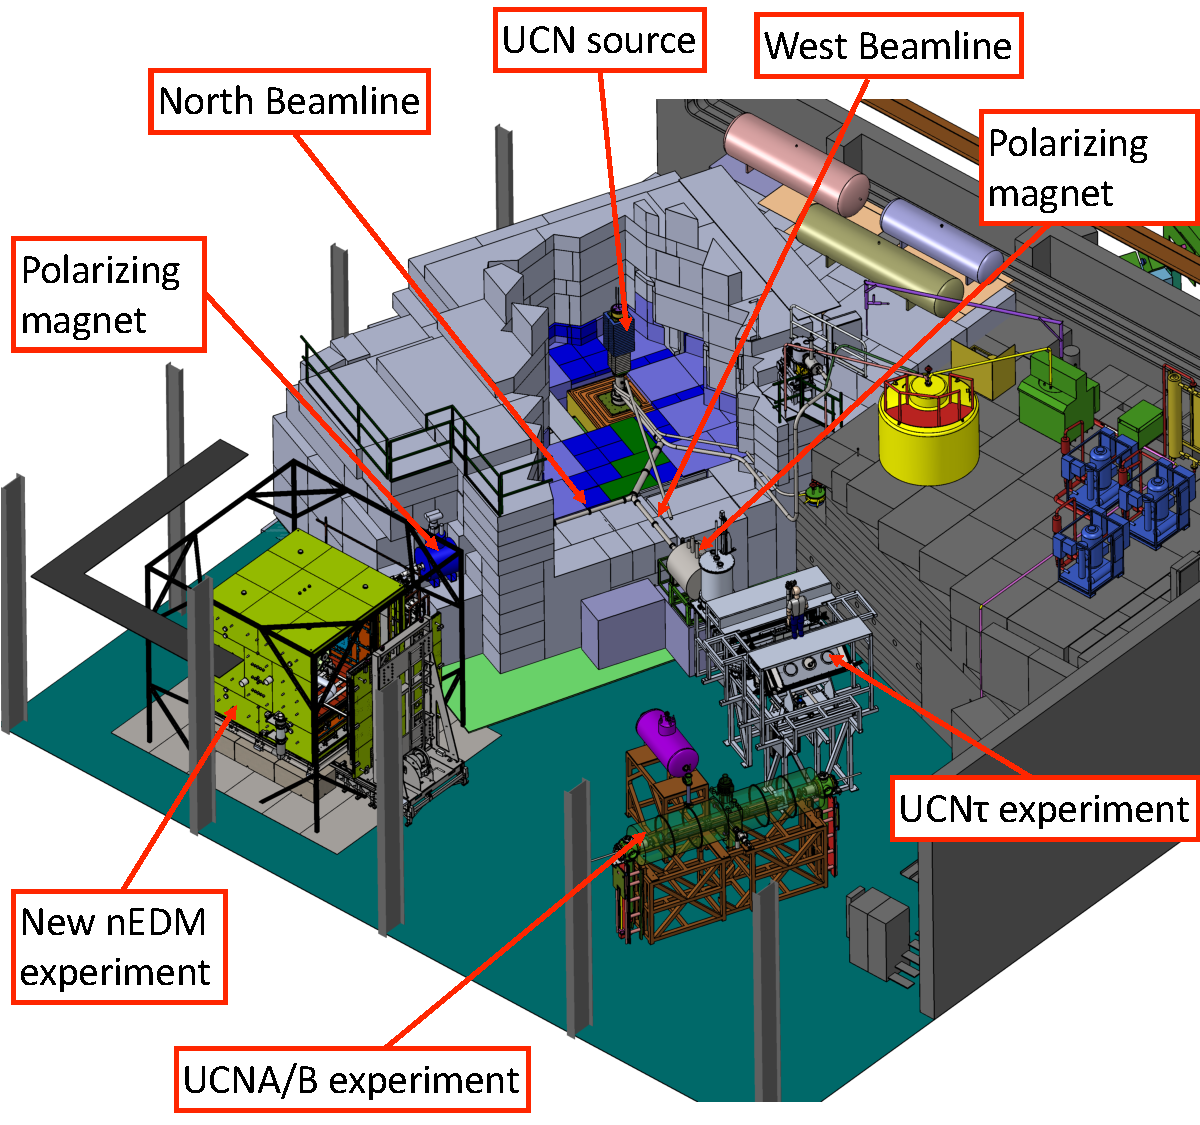
\includegraphics[width=0.6 \textwidth]{AreaB_v3.pdf}
    \caption{Schematic of the experimental area at the LANL UCN facility}
    \label{fig:AreaB_schematic}
\end{figure}

%%%%%%%%%%%%%%%%%%%%%%%%%%%%%%%%%%%%%%%%%

\section{Statistical uncertainty figure of merit}\label{sec:figure_of_merit}

%%%%%%%%%%%%%%%%%%%%%%%%%%%%%%%%%%%%%%%%%

Equation~7.28 from Ref.~\cite{golubUCN} gives the number of neutrons counted in a single Ramsey sequence as
%
\begin{gather}
    N_\text{R}(\Delta \omega) = N \left( 1 - \gls*{alpha} \cos \,\Delta \omega \, \gls*{T_fp} \right)/2
\end{gather}
%
where \gls*{alpha} is the spin contrast of a Ramsey fringe, defined by Eq.~(\ref{eq:alpha}), and $\gls*{T_fp}$ is the free precession period of the Ramsey method. A nonzero nEDM causes an interaction with $\vv{E}$ that produces a precession frequency shift $\Delta\omega=\omega-\omega_0$, where $\omega$ is the applied RF frequency and $\omega_0$ is defined by Eq.~(\ref{eq:larmor_freq}). 

To maximize sensitivity to small shifts in the resonant frequency, we examine where the slope of the central fringe is largest
%
\begin{gather}
    \frac{\partial N_\text{R}(\Delta \omega)}{\partial \, \Delta \omega} = N \frac{\alpha}{2} \gls*{T_fp} \sin \, \Delta \omega \, \gls*{T_fp} \label{eq:slope_ramsey}
\end{gather}
%
The error of $\Delta \omega$ is given by
%
\begin{gather}
    \sigma(\Delta \omega) = \frac{\partial \, \Delta \omega}{\partial N_\text{R}(\Delta \omega)}\delta N_\text{R}(\Delta \omega) = \frac{\partial \, \Delta \omega}{\partial N_\text{R}(\Delta \omega)} \sqrt{N}
    \label{eq:sigma_delta_omega}
\end{gather}
%
Using Eq.~(\ref{eq:slope_ramsey}) where $\Delta \omega \, \gls*{T_fp} = \pi/2$ (for the largest slope), Eq.~(\ref{eq:sigma_delta_omega}) becomes
%
\begin{gather}
    \sigma(\Delta \omega) = \frac{2}{\gls*{alpha} \gls*{T_fp} \sqrt{N}}
\end{gather}
%
From reversal of the electric field, Eq.~(\ref{eq:delta_omega_dipole_relation}), we remove the dependence on $\Delta\omega$ to obtain
%
\begin{gather}
    \sigma_{\gls*{d_n}} = \frac{\hbar}{2\gls*{alpha} E \gls*{T_fp} \sqrt{N}}\label{eq:figure_of_merit}
\end{gather}
%
This is the figure of merit for an nEDM experiment using the Ramsey method. \gls{hbar} is Planck’s constant, \gls{alpha} is a factor describing the spin contrast of a Ramsey fringe, $N$ is the number of the detected UCN, and $E$ is the strength of the applied electric field.

%%%%%%%%%%%%%%%%%%%%%%%%%%%%%%%%%%%%%%%%%

\subsection
{
    \texorpdfstring{Statistical Uncertainty of the \acrshort{lanl} \acrshort{nedm}}
                    {Statistical Uncertainty of the LANL nEDM}\label{sec:lanl_nedm_uncertainty}
}

%%%%%%%%%%%%%%%%%%%%%%%%%%%%%%%%%%%%%%%%%

The nominal run parameters for the LANL nEDM are $\gls*{T_fp}=180\text{ s and } E=12\text{ kV/cm}$. As will be shown in Chap.~\ref{chap:north_beamline_paper}, we have measured $N=60\,000\text{ counts per cell}$. We let $\gls*{alpha}=0.8$, as was achieved in Ref.~\cite{ABE20}.

Using Eq.~(\ref{eq:figure_of_merit}), the uncertainty per cell per run is $7.8 \times 10^{-25}e\cdot\text{cm}$. For a full day of measurements (assuming a \qty{300}{\s} duty cycle with two precession cells), we have $N_\text{day}=2\times60\,000\times86\,400\text{ (seconds in a day)}/300$ and $\sigma_{\gls*{d_n}}=3.24\times10^{-26}e\cdot\text{cm}$. A year of continuous running gives $N_\text{year}=365\times N_\text{day}$ and $\sigma_{\gls*{d_n}}=1.7\times10^{-27}e\cdot\text{cm}$. At a 90\% confidence level, the uncertainty is multiplied by an additional factor of $1.6$, giving
%
\begin{gather}
    \sigma_{\gls*{d_n}}=2.71\times10^{-27}e\cdot\text{cm (90\% \acrshort{cl})}
\end{gather}
%
With an assumed data taking efficiency of 50\% (for experiment down time, calibration and systematic studies) and the accelerator production schedule at LANL, this uncertainty would be reached in 5 calendar years.

%%%%%%%%%%%%%%%%%%%%%%%%%%%%%%%%%%%%%%%%%

\section
{
    \texorpdfstring{UCN production at \acrshort{lanl}}
                   {UCN production at LANL}
}\label{sec:lanl_ucn_source}

%%%%%%%%%%%%%%%%%%%%%%%%%%%%%%%%%%%%%%%%%

At LANL, neutrons are produced by a pulsed \qty{800}{M\eV} proton beam incident on a tungsten target, which is surrounded by ambient temperature beryllium and graphite. The spallation neutrons are cooled by polyethylene bead moderators to cold neutrons, and are then converted to UCN by downscattering within an SD$_2$ crystal~\cite{saunders_performance_2013}.

As in Fig.~\ref{fig:lanl_ucn_source}, UCN leaving the SD$_2$ crystal are directed upwards along a \qty{1}{\meter} vertical guide coated in $\ce{^{58}Ni}$, to account for a Snell's law \qty{100}{\nano\eV} boost (Sec.~\ref{sec:ucn_reflection_transmission}). The UCN are then transported \qty{6}{\meter} along a horizontal NiP coated stainless steel guide to the exit of the biological shield~\cite{ito_performance_2018}.

A butterfly valve near the bottom of the vertical guide reduces the probability of UCN returning to the SD$_2$ and being absorbed. The valve is open while proton beam pulses are delivered to the spallation target and closed otherwise. The proton current from the accelerator is delivered in packets of 10 pulses, of pulse width \qty{625}{\micro\s} at \qty{20}{\hertz}, with a gap between packets of \qty{5}{\s}. The average current delivered to the target is $\sim\qty{9}{\micro A}$.

In a 2017 source upgrade, the cryogenic insert, which housed the SD$_2$ converter as well as the cold neutron moderator, was replaced with an improved design. The upgrade produced a factor of four increase in UCN density. UCN density measured at the exit of the biological shield was $\qty{184(32)}{UCN\per \cm^3}$, and polarized UCN density stored in an external chamber was $\qty{39(7)}{UCN\per \cm^3}$~\cite{ito_performance_2018}.

With the upgrade, a new UCN beamline (called the North Beamline) was constructed for the new nEDM experiment (Fig.~\ref{fig:AreaB_schematic}). Measurements and analysis characterizing the performance of the North Beamline are presented in Chap.~\ref{chap:north_beamline_paper}.

\begin{figure}
    \centering
    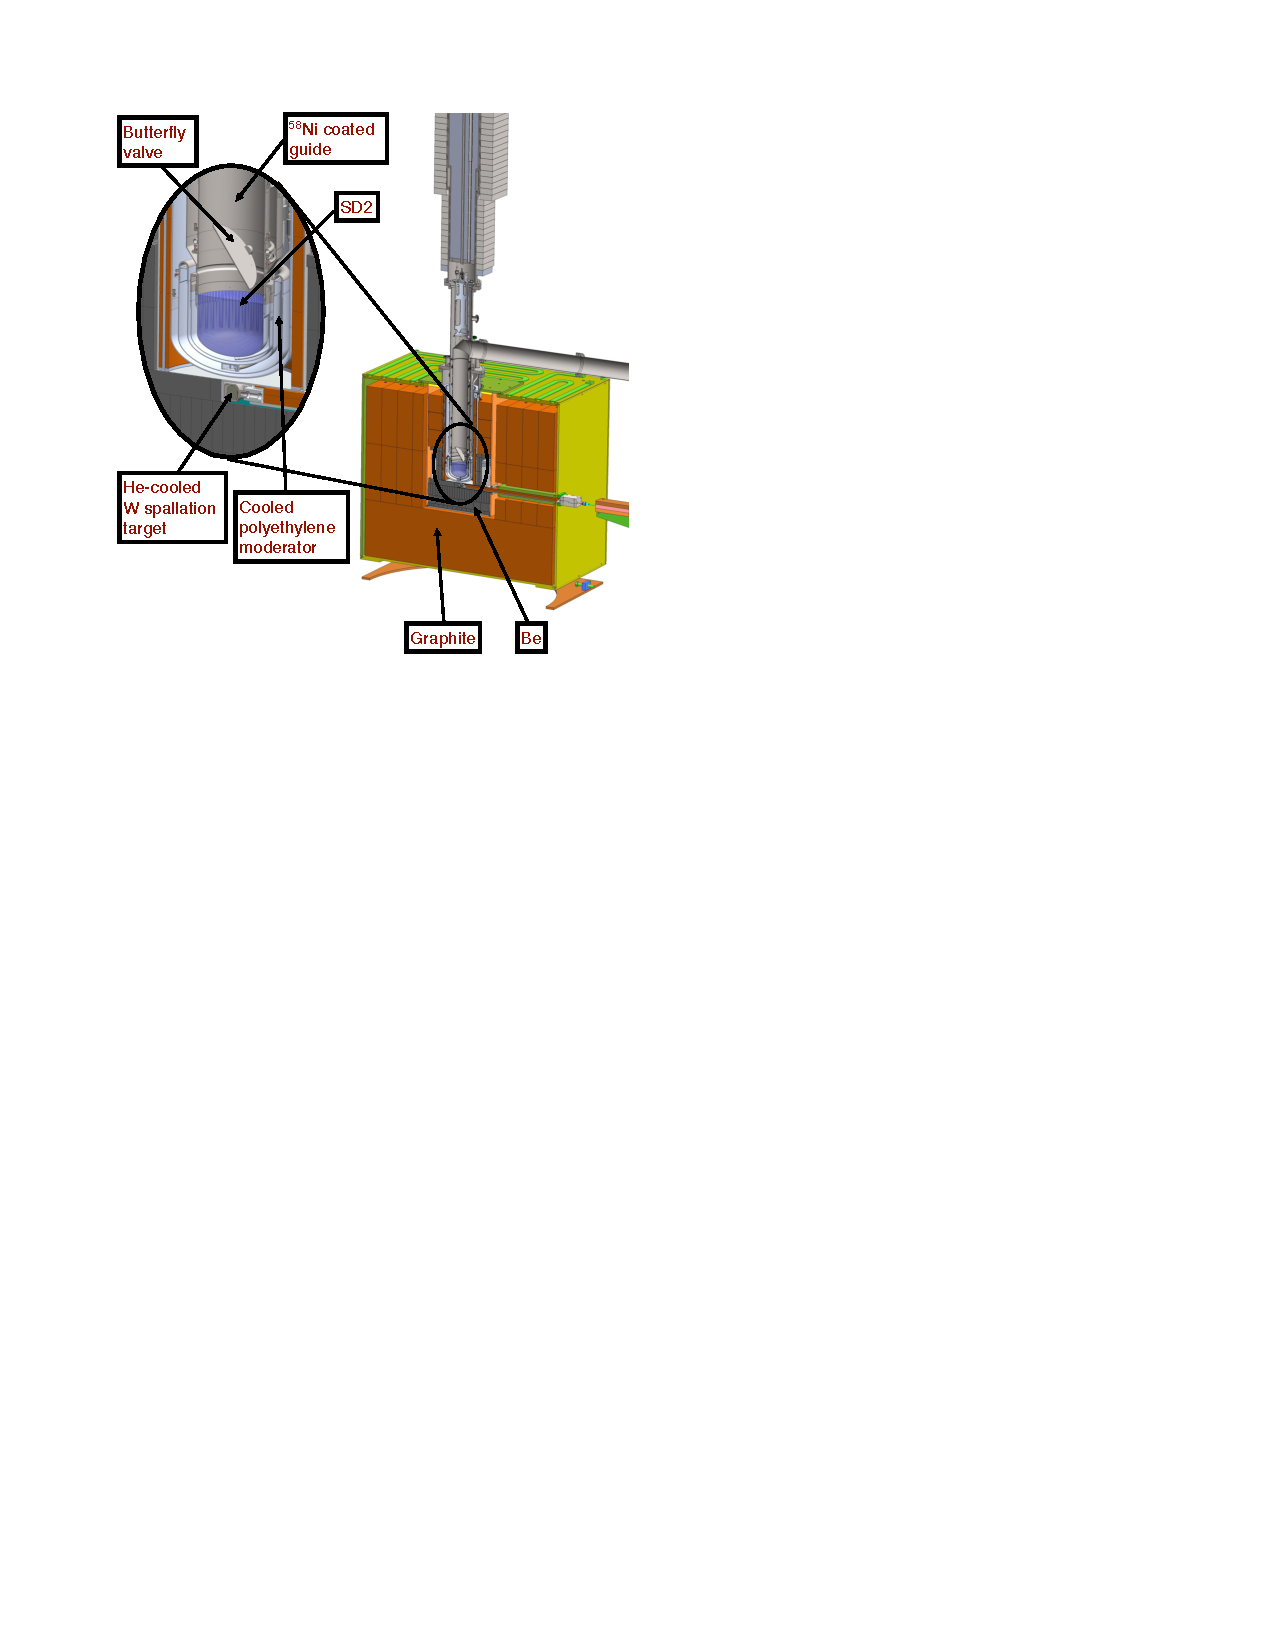
\includegraphics[width=0.45 \textwidth]{figures/lanl_ucn_source.pdf}
    \caption[Cutaway view of the LANL UCN source]
    {Cutaway view of the LANL UCN source. Image from Ref.~\cite{ito_performance_2018}}
    \label{fig:lanl_ucn_source}
\end{figure}


%%%%%%%%%%%%%%%%%%%%%%%%%%%%%%%%%%%%%%%%%

\section
{
    Magnetic field uniformity and stability requirements\label{sec:magnetic_field_req}
}

%%%%%%%%%%%%%%%%%%%%%%%%%%%%%%%%%%%%%%%%%

\comment{McGregor T2}

%%%%%%%%%%%%%%%%%%%%%%%%%%%%%%%%%%%%%%%%%

\subsection
{
    \texorpdfstring{$\ce{^{199}Hg}$ Comagnetometer}
                    {199Hg Comagnetometer}\label{sec:199hg_comag}
}

%%%%%%%%%%%%%%%%%%%%%%%%%%%%%%%%%%%%%%%%%

%%%%%%%%%%%%%%%%%%%%%%%%%%%%%%%%%%%%%%%%%

\subsection
{
    \texorpdfstring{$v\times E$ motional effect}
                    {v x E motional effect}\label{sec:v_cross_E}
}

%%%%%%%%%%%%%%%%%%%%%%%%%%%%%%%%%%%%%%%%%

A particle with velocity $\vv{v}$ moving in fields $\vv{E}$ and $\vv{B}_0$ sees in its rest frame a field $\vv{B}'$ given by
%
\begin{align}
    \vv{B}' &= \vv{B}_0+\vv{B}_{v\times E} \\
            &= \vv{B}_0-\gls{lorentz}\frac{\vv{v}\times\vv{E}}{c^2}
\end{align}
%
where the Lorentz factor $\gls*{lorentz}=\glsvalue*{lorentz}\approx 1$ for \ucn and cold neutron velocities. When compounded with other factors described in this section, this gives rise to false nEDM signals.

Again borrowing the form of Eq.~(\ref{eq:delta_omega_dipole_relation}), false nEDMs are generated from $E$-odd components of the frequency shifts do not disappear upon reversal of the $E$ field.
%
\begin{gather}
    d_\text{false}=\frac{\hbar}{4E}(\Delta\omega(E)-\Delta\omega(-E))
\end{gather}

\subsection*{
    \texorpdfstring{Nonparallel $E$ and $B$ fields}
                    {Nonparallel E and B fields}
}

We examine the false nEDM from misalignment of $E$ and $B$ fields in combination with the $v\times E$ effect. Let $\theta_{EB}$ be the angle between $\vv{E}$ and $\vv{B}_0$ in the plane perpendicular to $\vv{v}$. We can then write the frequency shift as~\cite{lamoreaux_experimental_2009}
%
\begin{align}
    B' &\approx B_0 + \theta_{EB} B_{v\times E} + \frac{B_{v\times E}^2}{2B_0}\\
    \Delta\omega_\text{false} &\approx -\gls{gamma_n}\left( \theta_{EB} B_{v\times E} + \frac{B_{v\times E}^2}{2B_0} \right) \\
    &\approx -\gls{gamma_n} \frac{\theta_{EB}v}{c}E 
\end{align}
%
where we keep only $E$-odd terms.

For cold neutron beam nEDM experiments (Sec.~\ref{sec:history_nedm}) this effect was quite substantial. For reference, the uncertainty of the most accurate beam nEDM experiment to date \cite{dress_nedm_1977} constrained $\theta_{EB}$ to $<\qty{1.1e-4}{rad}$, but was still limited by an uncertainty of $\sim 10^{-24}\,e\text{ cm}$. (To reduce the $v\times E$ effect, the experiment was even built on a naval gun turret mount to enable the reversal of $\vv{v}$ through the apparatus!) 

In contrast, nEDM experiments using stored \ucn gain the benefit of $\langle v \rangle =0$ for the neutron population. Assuming there is no persistent overall motion of the \ucn caused by the storage geometry, filling procedure, etc., the systematic effects of nonparallel $E$ and $B$ fields are negligible at current sensitivities. As discussed in Ref.~\cite{pendlebury_revised_2015}, demands on field alignment are significantly relaxed if reflections of \ucn off the walls of the storage cell are sufficiently nonspecular.

\subsection*{Geometric phase}

Inhomogenous magnetic fields transverse to $\vv{B}_0$ in combination with the $v\times E$ effect gives rise to the geometric phase effect, a large false nEDM signal at current sensitivities. 

Reference~\cite{pendlebury_geometric-phase-induced_2004} considers the often-cited example of a  magnetic ``barrel'' gradient with cylindrical symmetry and particles in roughly circular orbits about a storage cell.
%
\begin{gather}
    B_r(r)=\frac{r}{2}\frac{\partial B_z}{\partial z}
\end{gather}
%
The gradient and $v\times E$ effect produce a rotating field in the rest frame of the particle, resulting in a variant of the Bloch-Siegert shift (Sec.~\ref{sec:bloch-siegert}). The magnitude of the geometric phase shift is dependent on the ratio of the orbital-trajectory frequency of a particle to its Larmor precession frequency. Thus, slow moving \ucn (adiabatic) see a shift given by~\cite{pendlebury_geometric-phase-induced_2004, pendlebury_revised_2015}
%
\begin{gather}
    \Delta\omega_\text{false} = \frac{v^2_{xy}}{8\pi B_0^2 c^2}\frac{\partial B_z}{\partial z}E
\end{gather}
%
and the faster Hg comagetometer atoms (nonadiabatic) see
%
\begin{gather}
    \Delta\omega_\text{false} = \frac{\gamma^2R_\text{cell}^2}{16\pi  c^2}\frac{\partial B_z}{\partial z}E
\end{gather}
%
where $v_{xy}$ is the average transverse particle velocity, $\gamma$ is the gyromagnetic ratio of the particle, and $R_\text{cell}$ is the radius of the storage cell. The geometric-phase false nEDM contribution from Hg is $\sim 50$ times larger than the contribution from \ucn~\cite{pendlebury_revised_2015}.

Of course, particles are not limited to strictly circular orbits about a cylindrical storage chamber. In addition to using Monte Carlos simulations (such as in Ref.~\cite{pignol_magic_2019}), more general expressions for geometric phase have been derived. References~\cite{pignol_geometric_phase_2012, pignol_geometric_phase_2015} use a perturbative treatment of transverse field inhomogeneities to obtain
%
\begin{gather}
    \Delta\omega_\text{false} = \frac{\gamma^2}{2\pi c^2}\langle xB_x + yB_y \rangle E
\end{gather}
%
where $\langle ... \rangle$ denotes a volume average over a storage cell of arbitrary geometry.

A formalism of geometric phase shift in terms of velocity autocorrelation functions can be found in Refs.~\cite{lamoreaux_geometric_phase_2005, barabanov_geometric_phase_2006, swank_geometric_phase_2009}.
%
\begin{align}
    \Delta\omega_\text{false} &= -\frac{\gamma^2 E}{2c^2}\left( \frac{\partial B_y}{\partial y} S_y(\omega_0) + \frac{\partial B_z}{\partial z} S_z(\omega_0) \right) \\
    S_i(\omega_0) &= 2\int_{-\infty}^{\infty} \frac{\Psi_i(\omega)}{(\omega_0^2 - \omega^2)}d\omega \\
    \Psi_i(x) &= \langle v_i(t)v_i(t-x) \rangle = \int_{-\infty}^{\infty}\cos (\omega x) \Psi_i (\omega) d\omega
\end{align}

%%%%%%%%%%%%%%%%%%%%%%%%%%%%%%%%%%%%%%%%%

\subsection{Magnetic contamination}

%%%%%%%%%%%%%%%%%%%%%%%%%%%%%%%%%%%%%%%%%

%%%%%%%%%%%%%%%%%%%%%%%%%%%%%%%%%%%%%%%%%

\subsection
{
    \texorpdfstring{Magnetically Shielded Room}
                    {Magnetically Shielded Room}\label{sec:MSR}
}

%%%%%%%%%%%%%%%%%%%%%%%%%%%%%%%%%%%%%%%%%

\begin{figure}
    \centering
    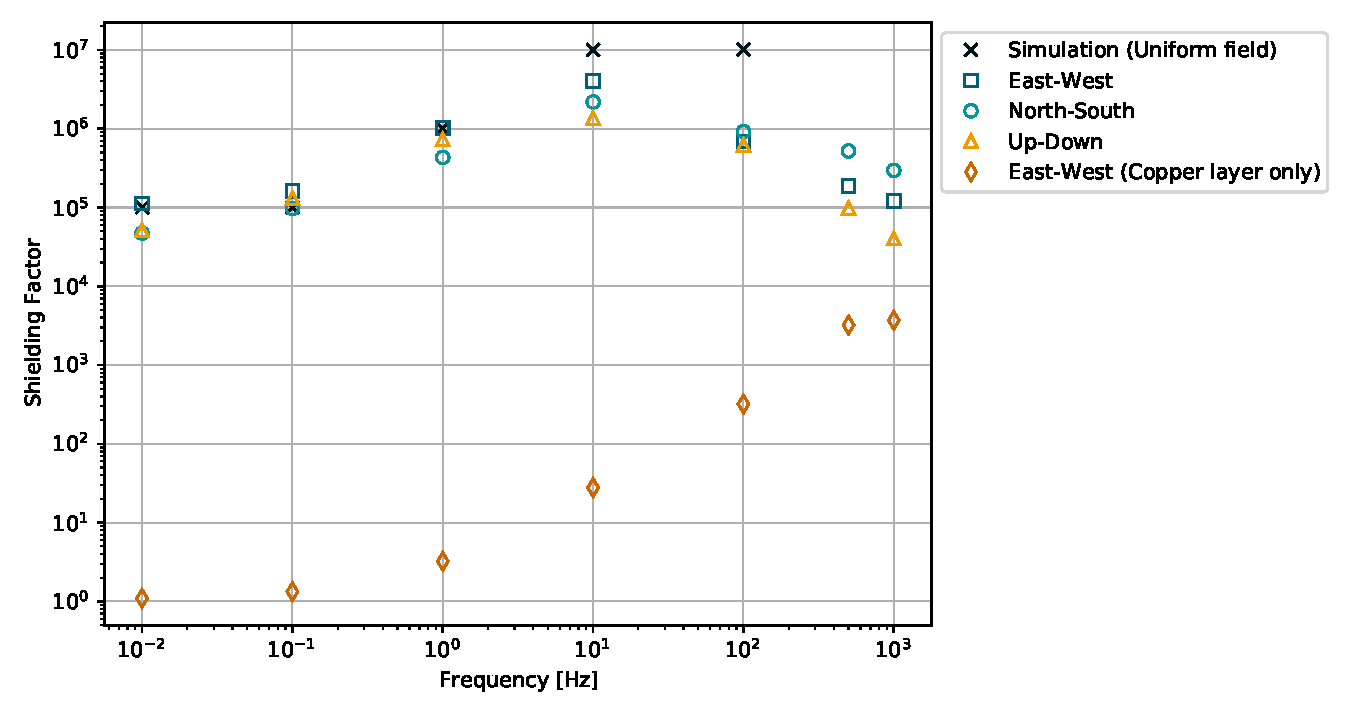
\includegraphics[width=\textwidth]{figures/chupp_msr_data.pdf}
    \caption
    {Shielding factor of the LANL nEDM MSR for various orientations excitation signal directions of an infinitely sized coil. See Sec.~\ref{sec:MSR} for methodology.}
    \label{fig:MSR-shielding-factor}
\end{figure}

A large magnetically shielded room (\acrshort*{msr}) is used for the attenuation of ambient external background magnetic fields. It has an overall shielding factor of $10^5$ for fields at frequency \qty{0.01}{\hertz} and a residual field of $<\qty{0.5}{nT}$.

The MSR consists of 4 Mumetal\textsuperscript{\textregistered} layers and one copper layer (Tab.~\ref{tb:lanl_msr_layers}). Mumetal\textsuperscript{\textregistered} is a magnetic shielding alloy ($\mu$-metal grade ASTM A753 Alloy 4, UNS N14080, 80NiFe) from the Magnetic Shield Corporation. The MSR utilizes a bolted construction to avoid welds that create magnetic domains. The frame of the MSR is stainless steel, which supports the load of the layers without deflection. The foundation of the MSR consists of high density aggregate precast blocks, minimizing the transmission of ambient external vibrations.

For optimized shielding performance, the ferromagnetic layers are degaussed periodically. Degaussing is done by applying an alternating field with large amplitude, which drives the material to saturation, and then slowly decreasing the amplitude to zero. Each $\mu$-metal layer contains multiple L-shaped coil sets, activated sequentially, for complete degaussing coverage (see Fig.~\ref{fig:degaussing-paper-cube} for the layout of coils on the innermost layer).

\comment{The LANL nEDM degaussing system uses an AC current supplied by an MCUSB-1808, which is then amplified by a custom (Gerard's) power supply...}

Residual magnetic fields in the degaussed \acrshort*{msr} were measured with a low noise 3-axis Bartington fluxgate probe (Tab.~\ref{tb:lanl_msr_dc_residuals}). The fluxgate was mounted on a glass fiber structure, and was inserted through the large neutron guide access tubes of the MSR. At each position, a \qty{10}{\second} measurement per fluxgate axis was taken in addition to a corresponding measurement where the fluxgate was rotated by \qty{180}{\degree}.

The absolute magnetic field values for an axis ($i=x,y,z$) were then calculated using the relations
%
\begin{align}
    B_{i,\text{ un-rotated}}&=\text{offset}+B_{i}\\
    B_{i,\text{ rotated}}&=\text{offset}-B_{i}\\
    \text{offset}&= (B_{i,\text{ un-rotated}} + B_{i,\text{ rotated}})/2
\end{align}
%
From the offset-corrected field values, the measured gradient upper limit was found to be $\qty{0.51}{nT\per m}$.

Shielding factor was determined by using the LANL field cage (Sec.~\ref{sec:field-cage}) to provide excitation signals. The resulting amplitude was measured with a fluxgate at the center of the MSR both before the start of MSR construction and after construction was completed. Excitation signals of amplitude \qty{1}{\micro\tesla} were used for frequencies \qty{0.01}{\hertz} and \qty{0.1}{\hertz}, \qty{10}{\micro\tesla} for \qty{1}{\hertz}, and \qty{30}{\micro\tesla} (max amplitude) for 10--\qty{1000}{\hertz}.

To account for the finite size of the excitation coil and the iron floor of the experimental area, finite-element physics simulations in COMSOL were used to obtain a scaling constant that related the field cage geometry shielding factor to an infinitely sized coil shielding factor. Shielding factors are shown in Fig.~\ref{fig:MSR-shielding-factor}.

\begin{table}
\centering
\caption{MSR layer composition}\label{tb:lanl_msr_layers}
\begin{tabular}{
    l
    c
    l
    S[table-format=1.2]
    c
    S[table-format=1.2]
    c
    S[table-format=1.2]
}
\toprule
Layer		& Thickness      & Material                        & \multicolumn{5}{c}{External side length}	\\
  &  {\scriptsize[mm]}    &  &  \multicolumn{5}{c}{$\text{\scriptsize [m}\scriptstyle\times \text{\scriptsize m}\scriptstyle\times\text{\scriptsize m]}$} \\
\midrule
1--outer	& 4  & Mumetal\textsuperscript{\textregistered}    & 3.5 & $\times$ & 3.5 & $\times$ & 3.5 \\
2	        & 3  & Mumetal\textsuperscript{\textregistered}    & 3.0 & $\times$ & 3.0 & $\times$ & 3.0 \\
3	        & 3  & Mumetal\textsuperscript{\textregistered}    & 2.6 & $\times$ & 2.6 & $\times$ & 2.6 \\
4	        & 8  & Copper                                      & 2.46 & $\times$ & 2.46 & $\times$ & 2.46 \\
5--inner	& 4  & Mumetal\textsuperscript{\textregistered}    & 2.39 & $\times$ & 2.39 & $\times$ & 2.39 \\
\bottomrule
\end{tabular}
% \end{table}
\vspace{\baselineskip}
% \begin{table}
% \centering
\caption{Residual DC fields in degaussed MSR}\label{tb:lanl_msr_dc_residuals}
\begin{tabular}{
    c
    S[table-format = 2.0]
    S[table-format = 2.0]
    S[table-format = 2.0]
    S[table-format = 1.2]
}
\toprule
Point		& $x$				& $y$				& $z$				& $|B|$	\\
{}    		& {\scriptsize(rel. to center)}	        & {\phantom{,,,}\scriptsize[cm]\phantom{,,,,}}       & {\scriptsize[cm]}		& {\scriptsize[nT]} 		\\
\midrule
1			& -40	            & -39	            & 23		        & 0.64\\
2			& 0	                & -39	            & 23	        	& 0.51\\
3			& 40                & -39	            & 23		        & 0.45\\
4			& -40	            & 39        		& -23	            & 0.52\\
5			& 0                 & 39        	    & -23	            & 0.41\\
6			& 40                & 39                & -23	            & 0.93\\
\bottomrule
\end{tabular}
\end{table}


\begin{figure}
    \centering
    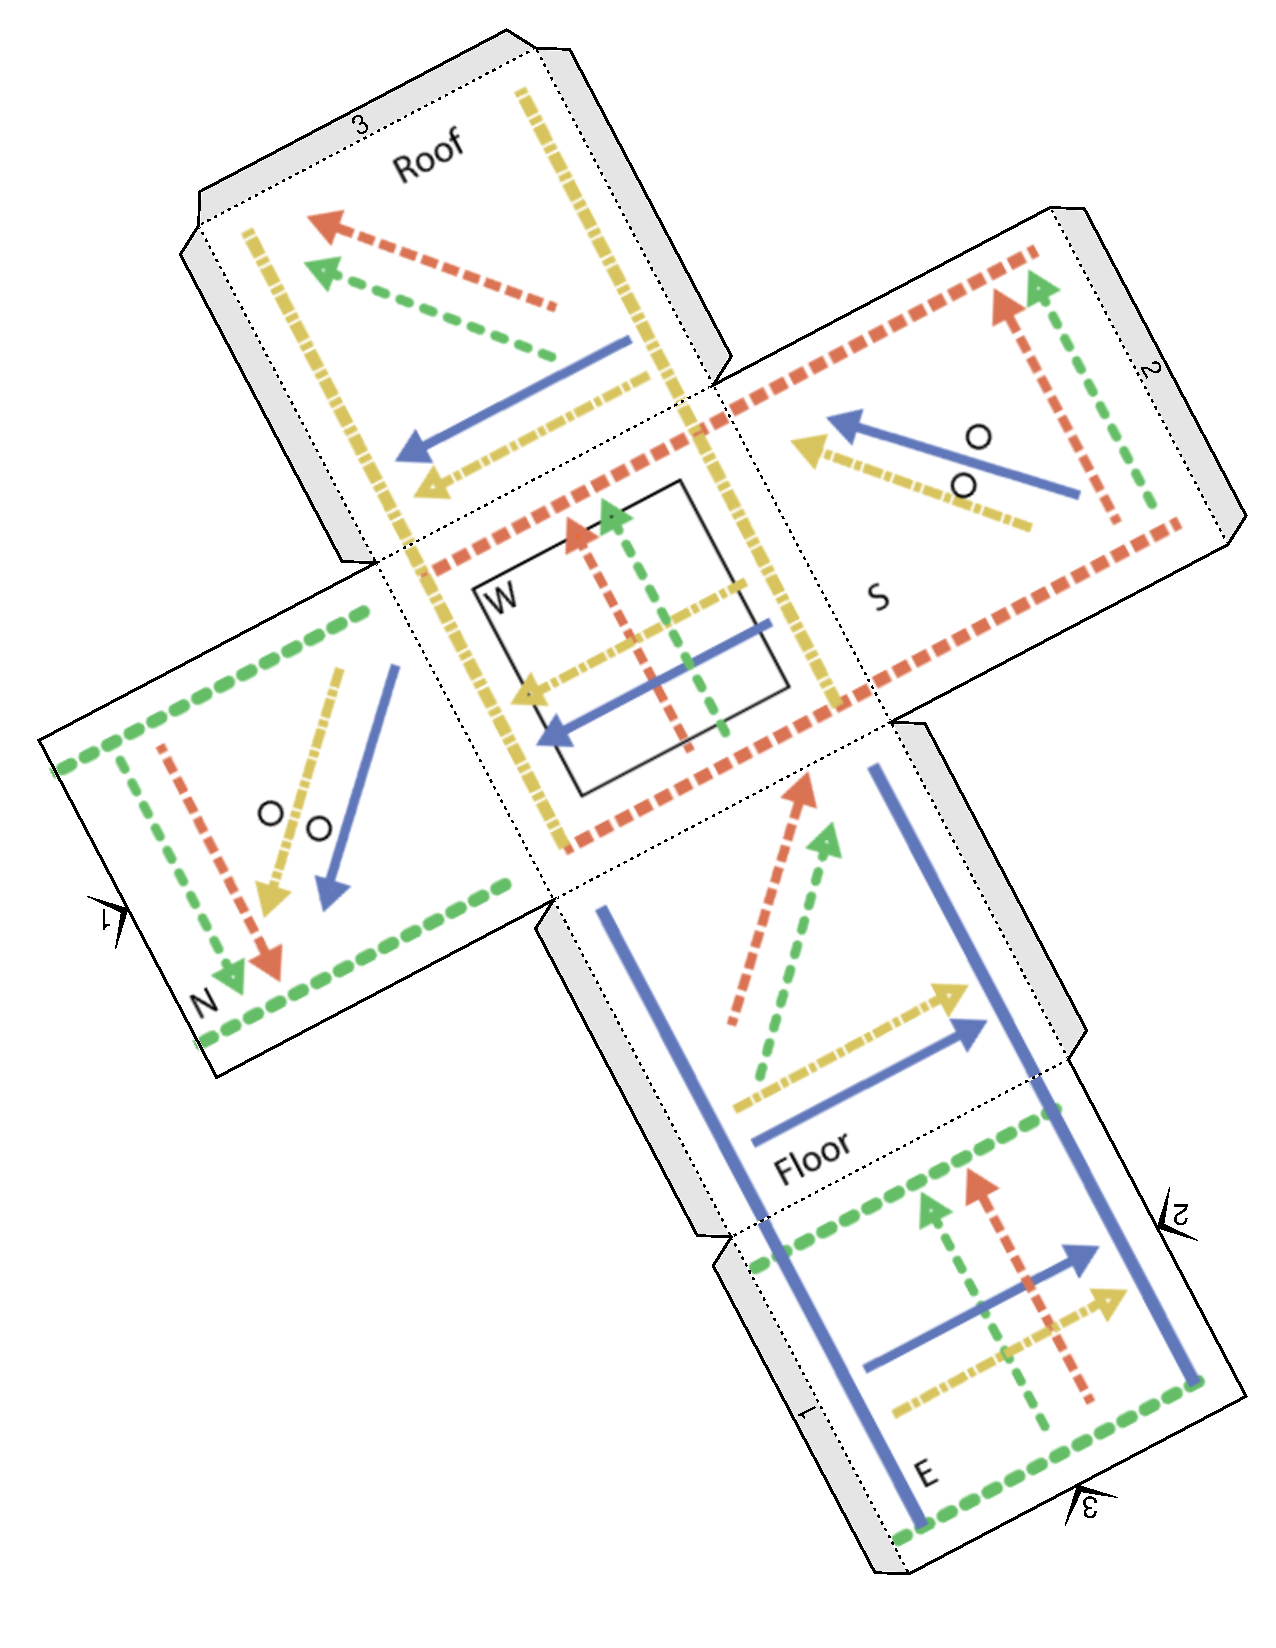
\includegraphics[width=\textwidth]{figures/L5-papercube.pdf}
    \caption
    {Simplified papercraft model of the four L-shaped degaussing coil sets on the innermost MSR layer and resulting flux contributions. Figure courtesy of Austin Reid.}
    \label{fig:degaussing-paper-cube}
\end{figure}

%%%%%%%%%%%%%%%%%%%%%%%%%%%%%%%%%%%%%%%%%

\subsection{External field active compensation}\label{sec:field-cage}

%%%%%%%%%%%%%%%%%%%%%%%%%%%%%%%%%%%%%%%%%

\begin{figure}
    \centering
    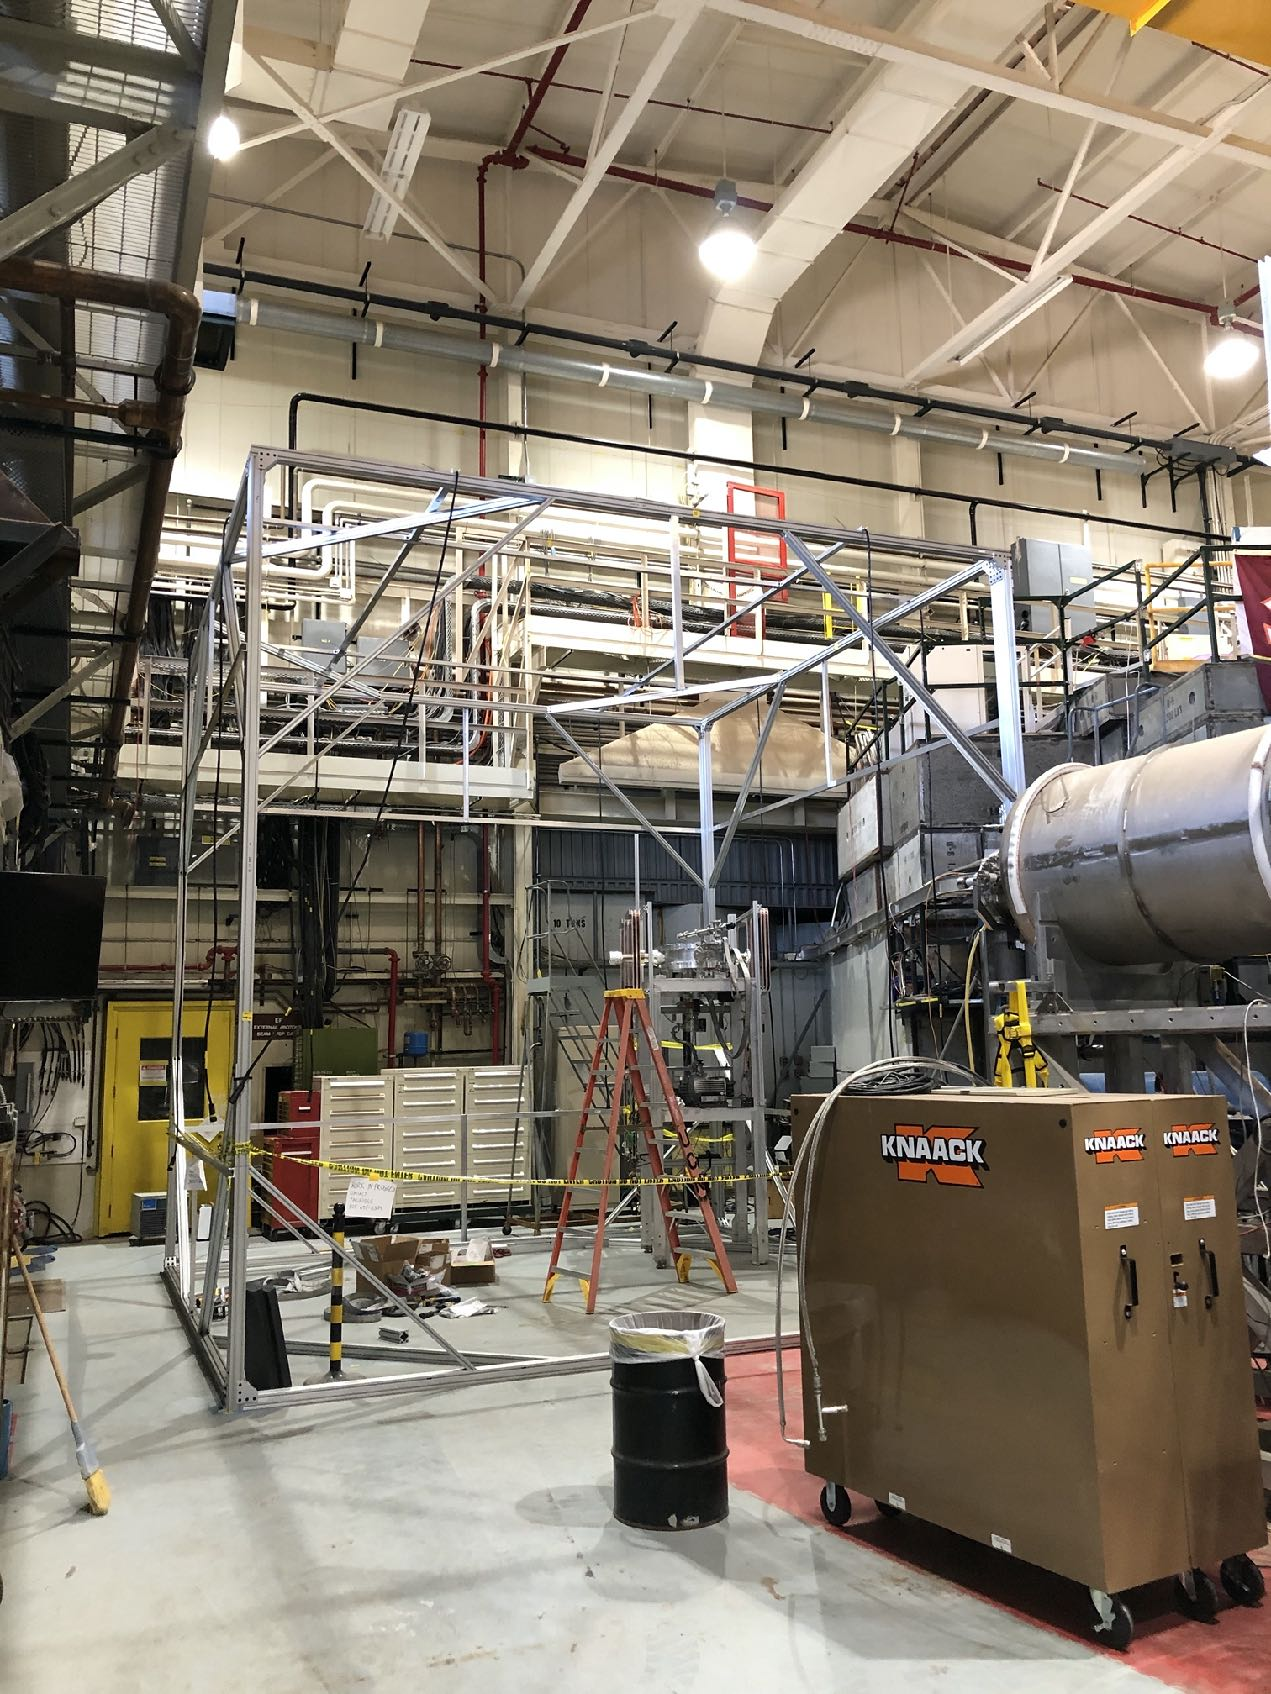
\includegraphics[height=4in]{figures/field_cage_no_msr.jpg}
    \caption
    {LANL nEDM field cage}
    \label{fig:lanl-field-cage}
\end{figure}

%%%%%%%%%%%%%%%%%%%%%%%%%%%%%%%%%%%%%%%%%

\subsection{
    \texorpdfstring{$B_0$ coil}
                {B0 coil}\label{sec:B0_coil}
}

%%%%%%%%%%%%%%%%%%%%%%%%%%%%%%%%%%%%%%%%%

%%%%%%%%%%%%%%%%%%%%%%%%%%%%%%%%%%%%%%%%%

\subsection{Transport coils}

%%%%%%%%%%%%%%%%%%%%%%%%%%%%%%%%%%%%%%%%%

%%%%%%%%%%%%%%%%%%%%%%%%%%%%%%%%%%%%%%%%%

\section{Additional sources of false nEDMs}

%%%%%%%%%%%%%%%%%%%%%%%%%%%%%%%%%%%%%%%%%


\subsection*{Leakage current}


\subsection*{Earth's rotation}


%%%%%%%%%%%%%%%%%%%%%%%%%%%%%%%%%%%%%%%%%

\section{Polarizing magnet}\label{sec:PM_description}

%%%%%%%%%%%%%%%%%%%%%%%%%%%%%%%%%%%%%%%%%

A \qty{5}{\tesla}, horizontal warm bore, superconducting magnet by American Magnetics Inc. is used as a polarizing magnet (\acrshort*{pm}). The PM field filters UCN spins, acting as a potential barrier that rejects low-field seeking UCN below \qty{300}{\nano\eV} and a potential well that passes high-field seeking UCN (Sec.~\ref{sec:ucn_polarizers}). 

A \qty{0.1}{\milli\meter} thick Al97 Mg3 alloy foil (similar in tensile strength to 6061-T6), termed the ``PM window," is located in the beamline at the center of the PM field region. This is used to separate the UCN source vacuum from the measurement apparatus vacuum, as the source vacuum can be routinely filled with D$_2$ gas (e.g. while D$_2$ is being drawn from a storage tank to be frozen or while SD$_2$ is being reconditioned). The magnetic potential of the PM overwhelms the neutron optical potential of the window (\qty{54}{\nano\eV} \cite{golubUCN}). The effect of the window on the transmission of UCN is discussed in detail in Sec.~\ref{sec:analysis}.

%%%%%%%%%%%%%%%%%%%%%%%%%%%%%%%%%%%%%%%%%

\section{Spin flipper and analyzers}\label{sec:spin_flipper_analyzer}

%%%%%%%%%%%%%%%%%%%%%%%%%%%%%%%%%%%%%%%%%

Neutron spin analyzers in the LANL nEDM are 10 layer polarizers made of iron and silicon located immediately above neutron detectors (see Ref.~\cite{ThorstenThesis} for layer structure details). When magnetized with a ($\sim \qty{10}{mT}$) field from permanent magnets, the multi-layer polarizer preferentially transmits high-field seeking UCN and rejects low-field seeking UCN with an analyzing power of $99.3^{+0.7}_{-2.4}\%$~\cite{ThorstenThesis}.

Note that it is not clear if the neutron energy spectrum under which Ref.~\cite{ThorstenThesis} is consistent with the LANL nEDM neutron spectrum. Reference~\cite{afach_device_2015} quotes an analyzing power of 95\% for a different but similar analyzing foil for an energy range of 90~neV to 330~neV, which includes the energy range of the UCN at the analyzing foil for the experiment reported in Sec.~\ref{sec:analysis}.

Additionally, an adiabatic fast passage (\acrshort{afp}) spin flipper coil, located upstream of the spin analyzer, is used to provide the option of spin flipping UCN (Sec.~\ref{sec:afp}). A schematic of the analyzer system is illustrated in Fig.~\ref{fig:SpinAnalyzer}.

\begin{figure}
    \centering
    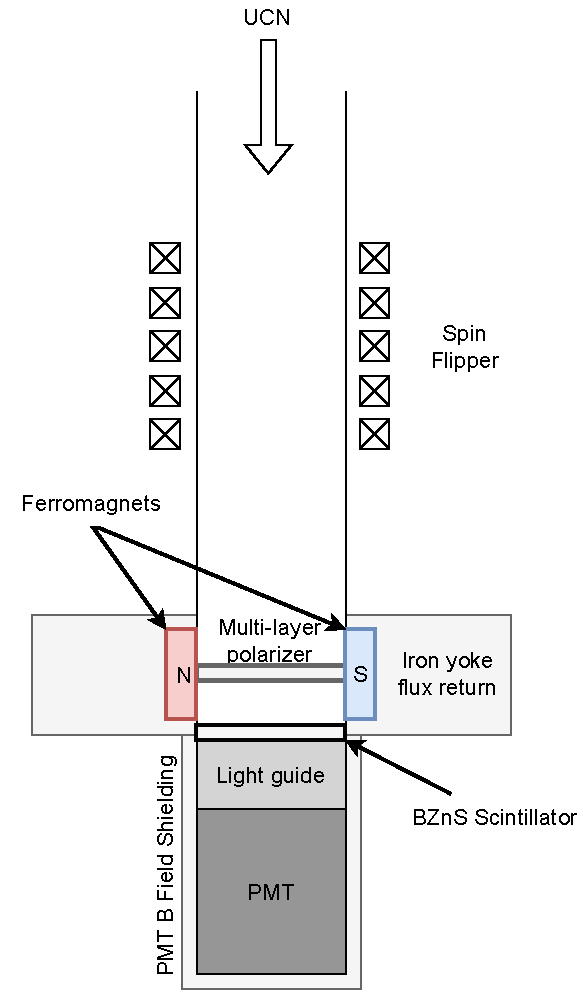
\includegraphics[width=5cm]{spinAnalyzer.pdf}
    \caption{Schematic of the adiabatic fast passage (\acrshort{afp}) spin flipper, spin analyzer, and UCN drop detector}
    \label{fig:SpinAnalyzer}
\end{figure}

%%%%%%%%%%%%%%%%%%%%%%%%%%%%%%%%%%%%%%%%%

\section{UCN detectors}\label{sec:ucn_detectors}

%%%%%%%%%%%%%%%%%%%%%%%%%%%%%%%%%%%%%%%%%

$\ce{^{10}B}$ coated ZnS:Ag scintillator films are used for UCN detection \cite{jeph_b10_2011}. UCN are captured on the top layer of $\ce{^{10}B}$, and reaction products ($^4$He and/or $^7$Li) from the $\ce{^{10}B}(\text{n},\alpha)^7\text{Li}$ neutron capture reaction are detected in the ZnS:Ag layer. The resulting scintillation light is then detected by a photomultiplier tube (\acrshort*{pmt}) or silicon photomultiplier (\acrshort*{sipm}).

%%%%%%%%%%%%%%%%%%%%%%%%%%%%%%%%%%%%%%%%%

\section{UCN switchers}

%%%%%%%%%%%%%%%%%%%%%%%%%%%%%%%%%%%%%%%%%

%%%%%%%%%%%%%%%%%%%%%%%%%%%%%%%%%%%%%%%%%

\section{Vacuum chamber}

%%%%%%%%%%%%%%%%%%%%%%%%%%%%%%%%%%%%%%%%%

%%%%%%%%%%%%%%%%%%%%%%%%%%%%%%%%%%%%%%%%%

\section{Precession chambers}\label{sec:precession_chambers}

%%%%%%%%%%%%%%%%%%%%%%%%%%%%%%%%%%%%%%%%%

\comment{Copy DLC coating procedure over from North beamline paper chap}

\comment{Mention large upstream volume}

%%%%%%%%%%%%%%%%%%%%%%%%%%%%%%%%%%%%%%%%%

\subsection{dPS coating procedure}\label{sec:dPS_coating}

%%%%%%%%%%%%%%%%%%%%%%%%%%%%%%%%%%%%%%%%%

\begin{figure}
\centering
%subfigure width gets "multiplied" by includegraphics width
\begin{subfigure}{.5\textwidth} 
  \centering
  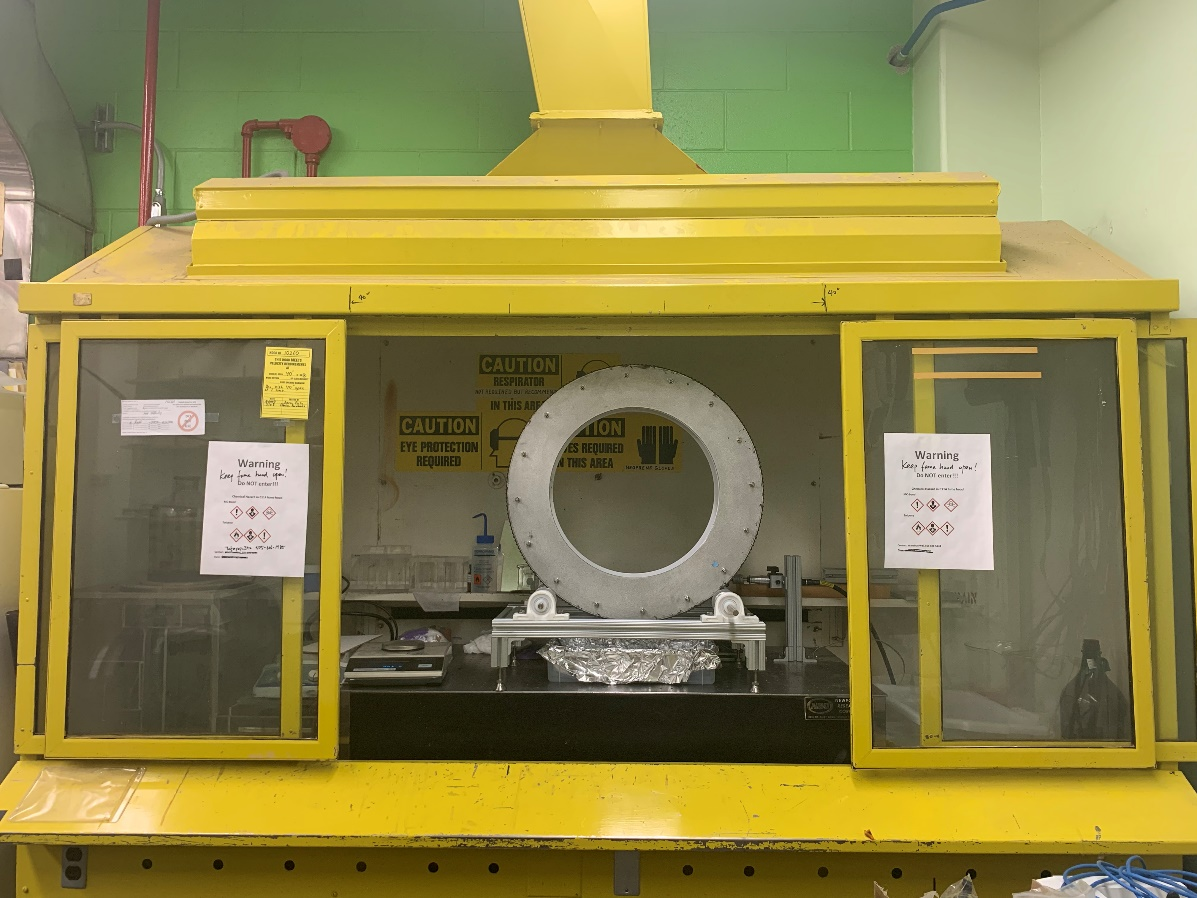
\includegraphics[width=\textwidth]{figures/dPS_jig_and_fume_hood.jpg}
\end{subfigure}%DO NOT REMOVE THIS '%'
\begin{subfigure}{.5\textwidth}
  \centering
  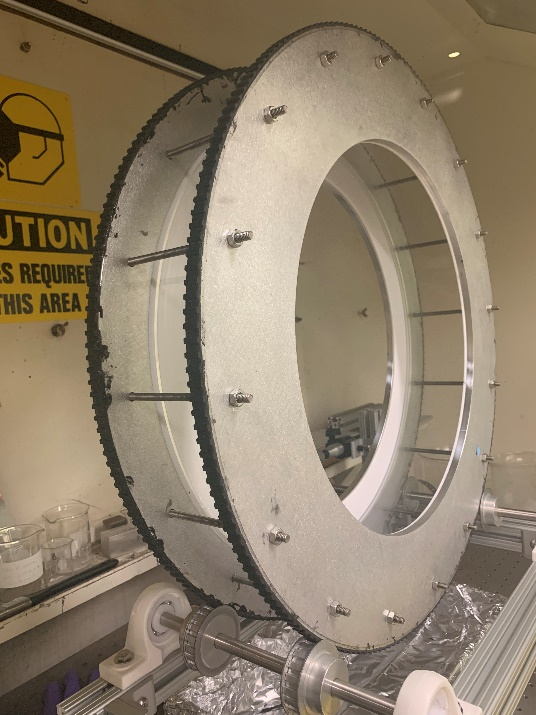
\includegraphics[width=0.57\textwidth]{figures/dPS_jig.jpg}
\end{subfigure}
\caption
{Precession cell wall coating jig, as described in Sec.~\ref{sec:dPS_coating}}
\label{fig:dPS_coating_jig}
\end{figure}